\subsection{A használt software-ek}

A CI/CD folyamat központi komponense a Drone CI platform. Több verziókezelő felülettel is kínál integrációt, ezek közül a Gitea-t használtam. A deploymentet a Portainer végzi.

A választott eszközöknél szempont volt, hogy ne legyen nagy az erőforrás-igényük, ugyanis a szerveren fut a teljes ELK-stack, és mindössze 4GB RAM és 2 processzor áll rendelkezésre.
Mindhárom tool Go nyelven íródott, amellyel ilyen jellegű eszközök esetén jó tapasztalatom volt, és a dokumentációkban kiemelik az erőforrás-hatékonyságukat (ellenben pl a Jenkins Java-s megoldásával, amely potenciálisan nagy memóriahasználattal jár).


\begin{figure}[H]
	\centering
	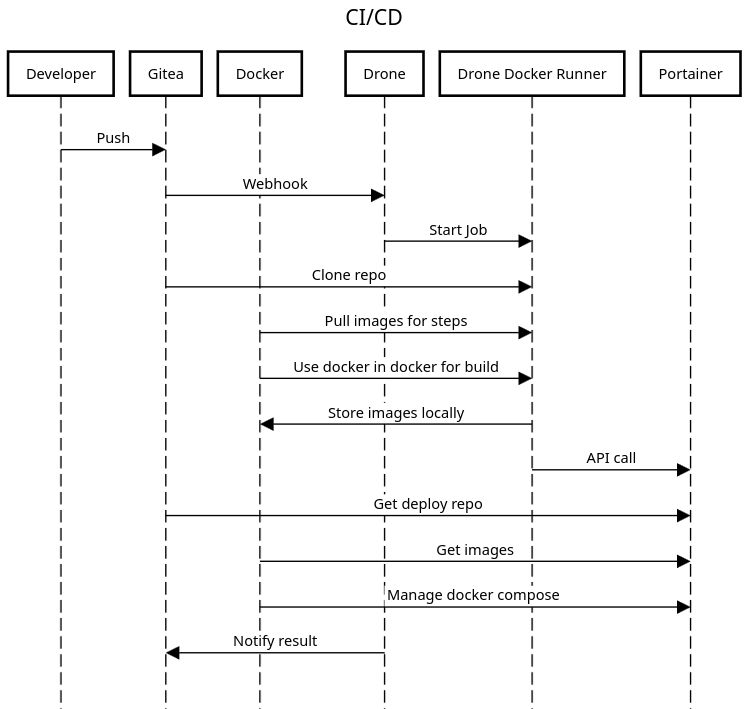
\includegraphics[width=0.9\linewidth]{img/seq.png}
	\caption{Szekvencia-diagram a teljes CI/CD folyamatról}
	\label{fig:seq}
\end{figure}


\newpage

\subsection{Hálózat}

Mivel nyilvánosan elérhető domain név nem állt a rendelkezésemre, a 
komponensek portjait megnyitottam a host gépre, és azokat a sajátomra port-forwarddal továbbítottam. A 8100-as portokat választottam a projekt számára.

A komponensek, amikor lehet, a Dockerben létrehozott hálózaton kommunikálnak egymással.

\begin{lstlisting}
$ cat ~/.ssh/config
Host chirpstack
    User ubuntu
    Hostname 164.30.6.180
    PreferredAuthentications publickey
    IdentityFile ~/.ssh/lora_rsa
    AddKeysToAgent yes

    LocalForward 8100 127.0.0.1:8100
    LocalForward 8101 127.0.0.1:8101
    LocalForward 8122 127.0.0.1:8122
    LocalForward 8102 127.0.0.1:8102
    LocalForward 8103 127.0.0.1:8103
    LocalForward 8104 127.0.0.1:8104
\end{lstlisting}

A hálózat definíciója, és a portok:

\begin{lstlisting}
services:
  portainer:
    ...
    ports:
      - 8100:9000
    networks:
      - infranet

  gitea:
    ...
    ports:
      - 8101:3000
      - 8122:22
    networks:
      - infranet

  drone:
    ...
    ports:
      - "8102:80"
    networks:
      - infranet

  drone-runner:
    ...
    networks:
      - infranet

networks:
  infranet:

\end{lstlisting}

A további két portot a példaképp kitelepített service fogja használni:
\begin{lstlisting}
services:
  lorawan-sniffer-test:
    ...
    ports:
      - 8103:8000
      - 8104:8001
\end{lstlisting}

Ahol a 8000-es port a REST API interface, a 8001 pedig a Prometheus metrikák.

\subsection{Perzisztálás}

A hosszútávú, újraindulásokon átívelő adattárolás megoldására bind mount-okat alkalmaztam, mivel ezek pontos helye kényelmesebben megtalálható, mint a volume-ok esetében.

Valamint szükség volt a Docker unix socket mount-olására is, mivel több container is használja azt saját működése során.

Az infrastruktúra komponensek:

\begin{lstlisting}
services:
  portainer:
    ...
      - /var/run/docker.sock:/var/run/docker.sock
      - $DATA_DIR/$COMPOSE_PROJECT_NAME/portainer/data:/data
    
  gitea:
    ...
      - $DATA_DIR/$COMPOSE_PROJECT_NAME/gitea/data:/data

  drone:
    ...
    volumes:
      - $DATA_DIR/$COMPOSE_PROJECT_NAME/drone/data:/data
    
  drone-runner:
    volumes:
      - /var/run/docker.sock:/var/run/docker.sock

\end{lstlisting}

A demo alkalmazás configjait szintén mount-olom:

\begin{lstlisting}
services:
  lorawan-sniffer-test:
    volumes:
      - $PORTAINER_STACKS_DIR/$PORTAINER_STACK_ID/lorawan-sniffer/config.toml:/app/config.toml
      - $PORTAINER_STACKS_DIR/$PORTAINER_STACK_ID/logging.toml:/app/logging.toml
\end{lstlisting}

Itt, mivel a Portainer maga is container-ként fut, nem triviális a relatív elérési úttal történő mountolás, ezért az abszolút az ajánlott. Az itt megadott elérési út a Portainer által kezelt Compose környezetek (Stack-ek) filerendszerbeli elhelyezésének logikáját követi le.


Az infra komponensek perzisztált adatai:
\begin{lstlisting}
ubuntu@chirpstack:~$ ls .data/infra/**/*
.data/infra/drone/data:
database.sqlite

.data/infra/gitea/data:
git  gitea  ssh

.data/infra/portainer/data:
bin  certs  chisel  compose  docker_config  portainer.db..
..portainer.key  portainer.pub  tls

\end{lstlisting}

\subsection{Portainer}

A Portainer egy webes felületet nyújt egy (vagy több) szerver Dockerhez köthető aktivitásának felügyeletére, működtetésére.

A projekt megvalósításához kettő Docker compose környezetet használok, ezeket a Portainer stack-nek 
hívja. Az első stack az infrastruktúra komponenseket tartalmazza. Ennek a leíróját git repóban tárolom, deploy-infra néven, amit kézzel juttatok el és frissítek a szerveren. A második a CI/CD folyamat által kezelt környezet, melyet a Portainer szerez be a verziókezelőből (deploy-demo néven), frissíti azt, és manage-eli a demo célból ott található service-t. 

Hogy képes legyen kezelni a Docker-t, fel kell mount-olni a Docker socketet:
\begin{lstlisting}
  portainer:
    ...
    volumes:
      - /var/run/docker.sock:/var/run/docker.sock
\end{lstlisting}

\newpage

Az infra környezet:

\begin{lstlisting}
ubuntu@chirpstack:~/docker/deploy-infra$ docker compose ps
NAME           IMAGE                           COMMAND
drone          drone/drone:2                   "/bin/drone-server"
drone-runner   drone/drone-runner-docker:1     "/bin/drone-runner-d…"
gitea          gitea/gitea:1.25.5              "/usr/bin/entrypoint…"
portainer      portainer/portainer-ce:2.39.0   "/portainer -H unix:…"
\end{lstlisting}

\begin{figure}[H]
	\centering
	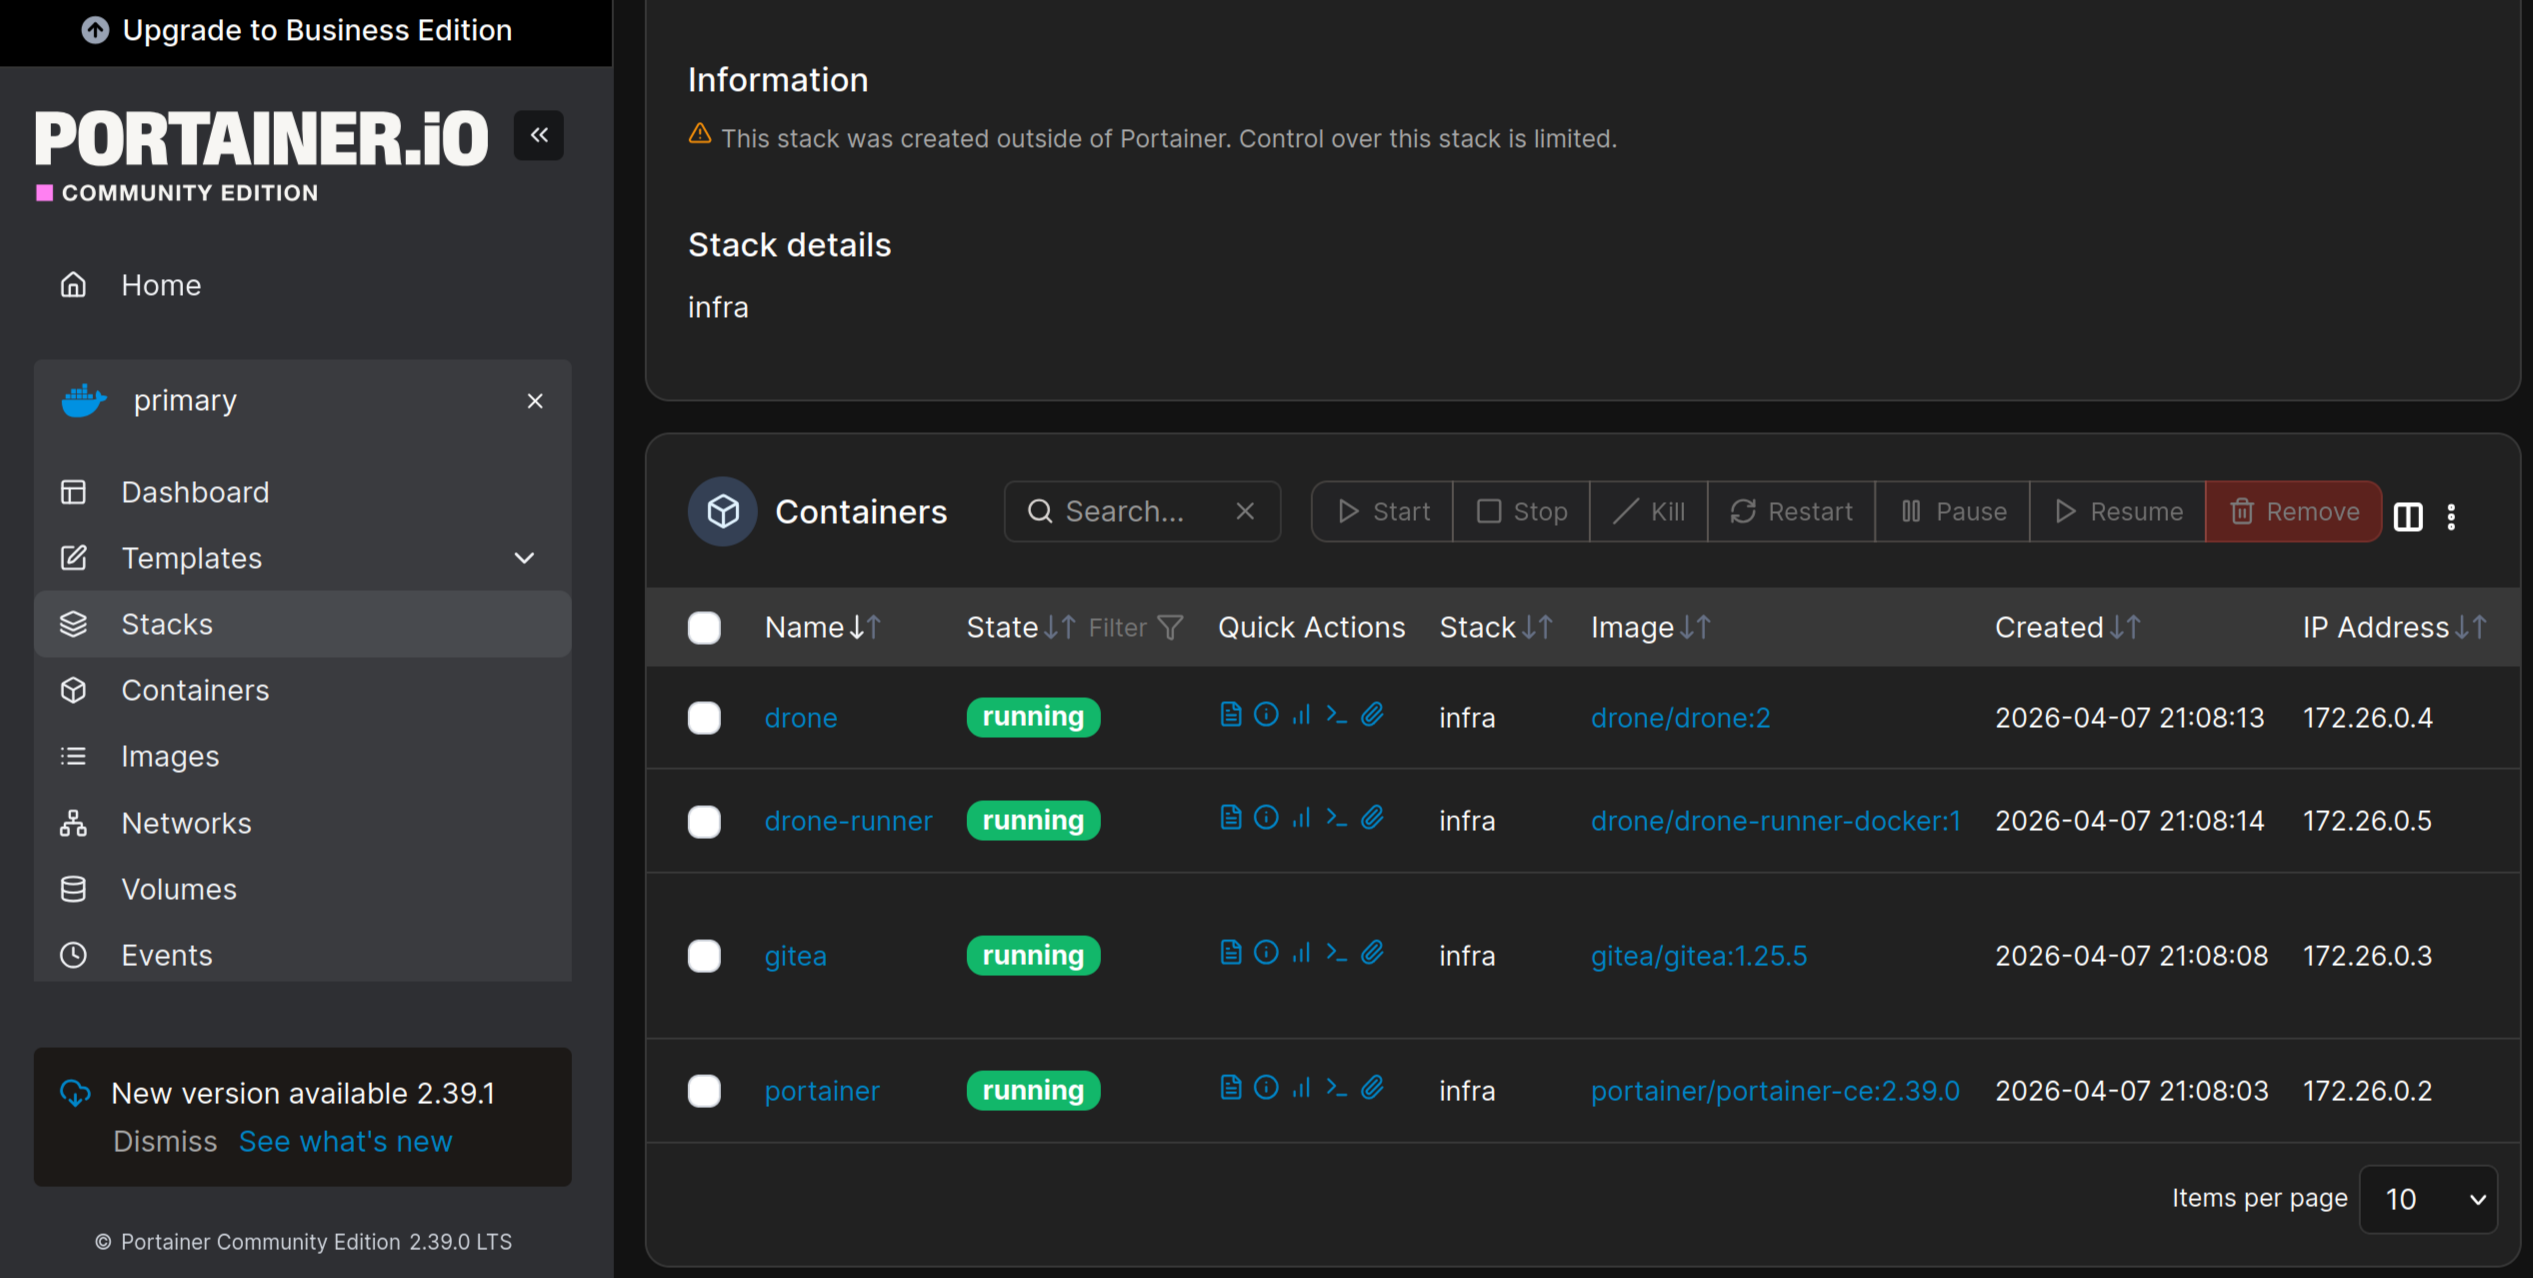
\includegraphics[width=1\linewidth]{img/portainer_infra.png}
	\caption{Az Infrastruktúra stack a Portainer GUI-n}
	\label{fig:seq}
\end{figure}


\subsection{Gitea}

A kutatócsoport alapvetően a GitHub-ra dolgozik, azonban az automatizációhoz szükséges, hogy a Drone CI-t meg tudja hívni a Git platform webhook hívással. Domain név hiányában egy lokálisan elérhető, saját platform futtatása mellett döntöttem, mely tovább bővítette a felhasznált Docker service-ek sorát.

Ahhoz, hogy a Gitea felülettel interaktálni tudjak, további ssh konfiguráció szükséges:

\begin{lstlisting}
szepesisz@neo:~$ cat ~/.ssh/config
 ...
    Host gitea
    User git
    Hostname localhost
    Port 8122
    PreferredAuthentications publickey
    IdentityFile ~/.ssh/gitea
\end{lstlisting}

Valamint a repository-nál:

\begin{lstlisting}
szepesisz@neo:~/Documents/OE/lora/LoRaWAN-sniffer$ git remote add gitea git@gitea:oe-lorawan/oe-lorawan-sniffer.git

szepesisz@neo:~/Documents/OE/lora/LoRaWAN-sniffer$ git pull gitea develop 
\end{lstlisting}

\begin{figure}[H]
	\centering
	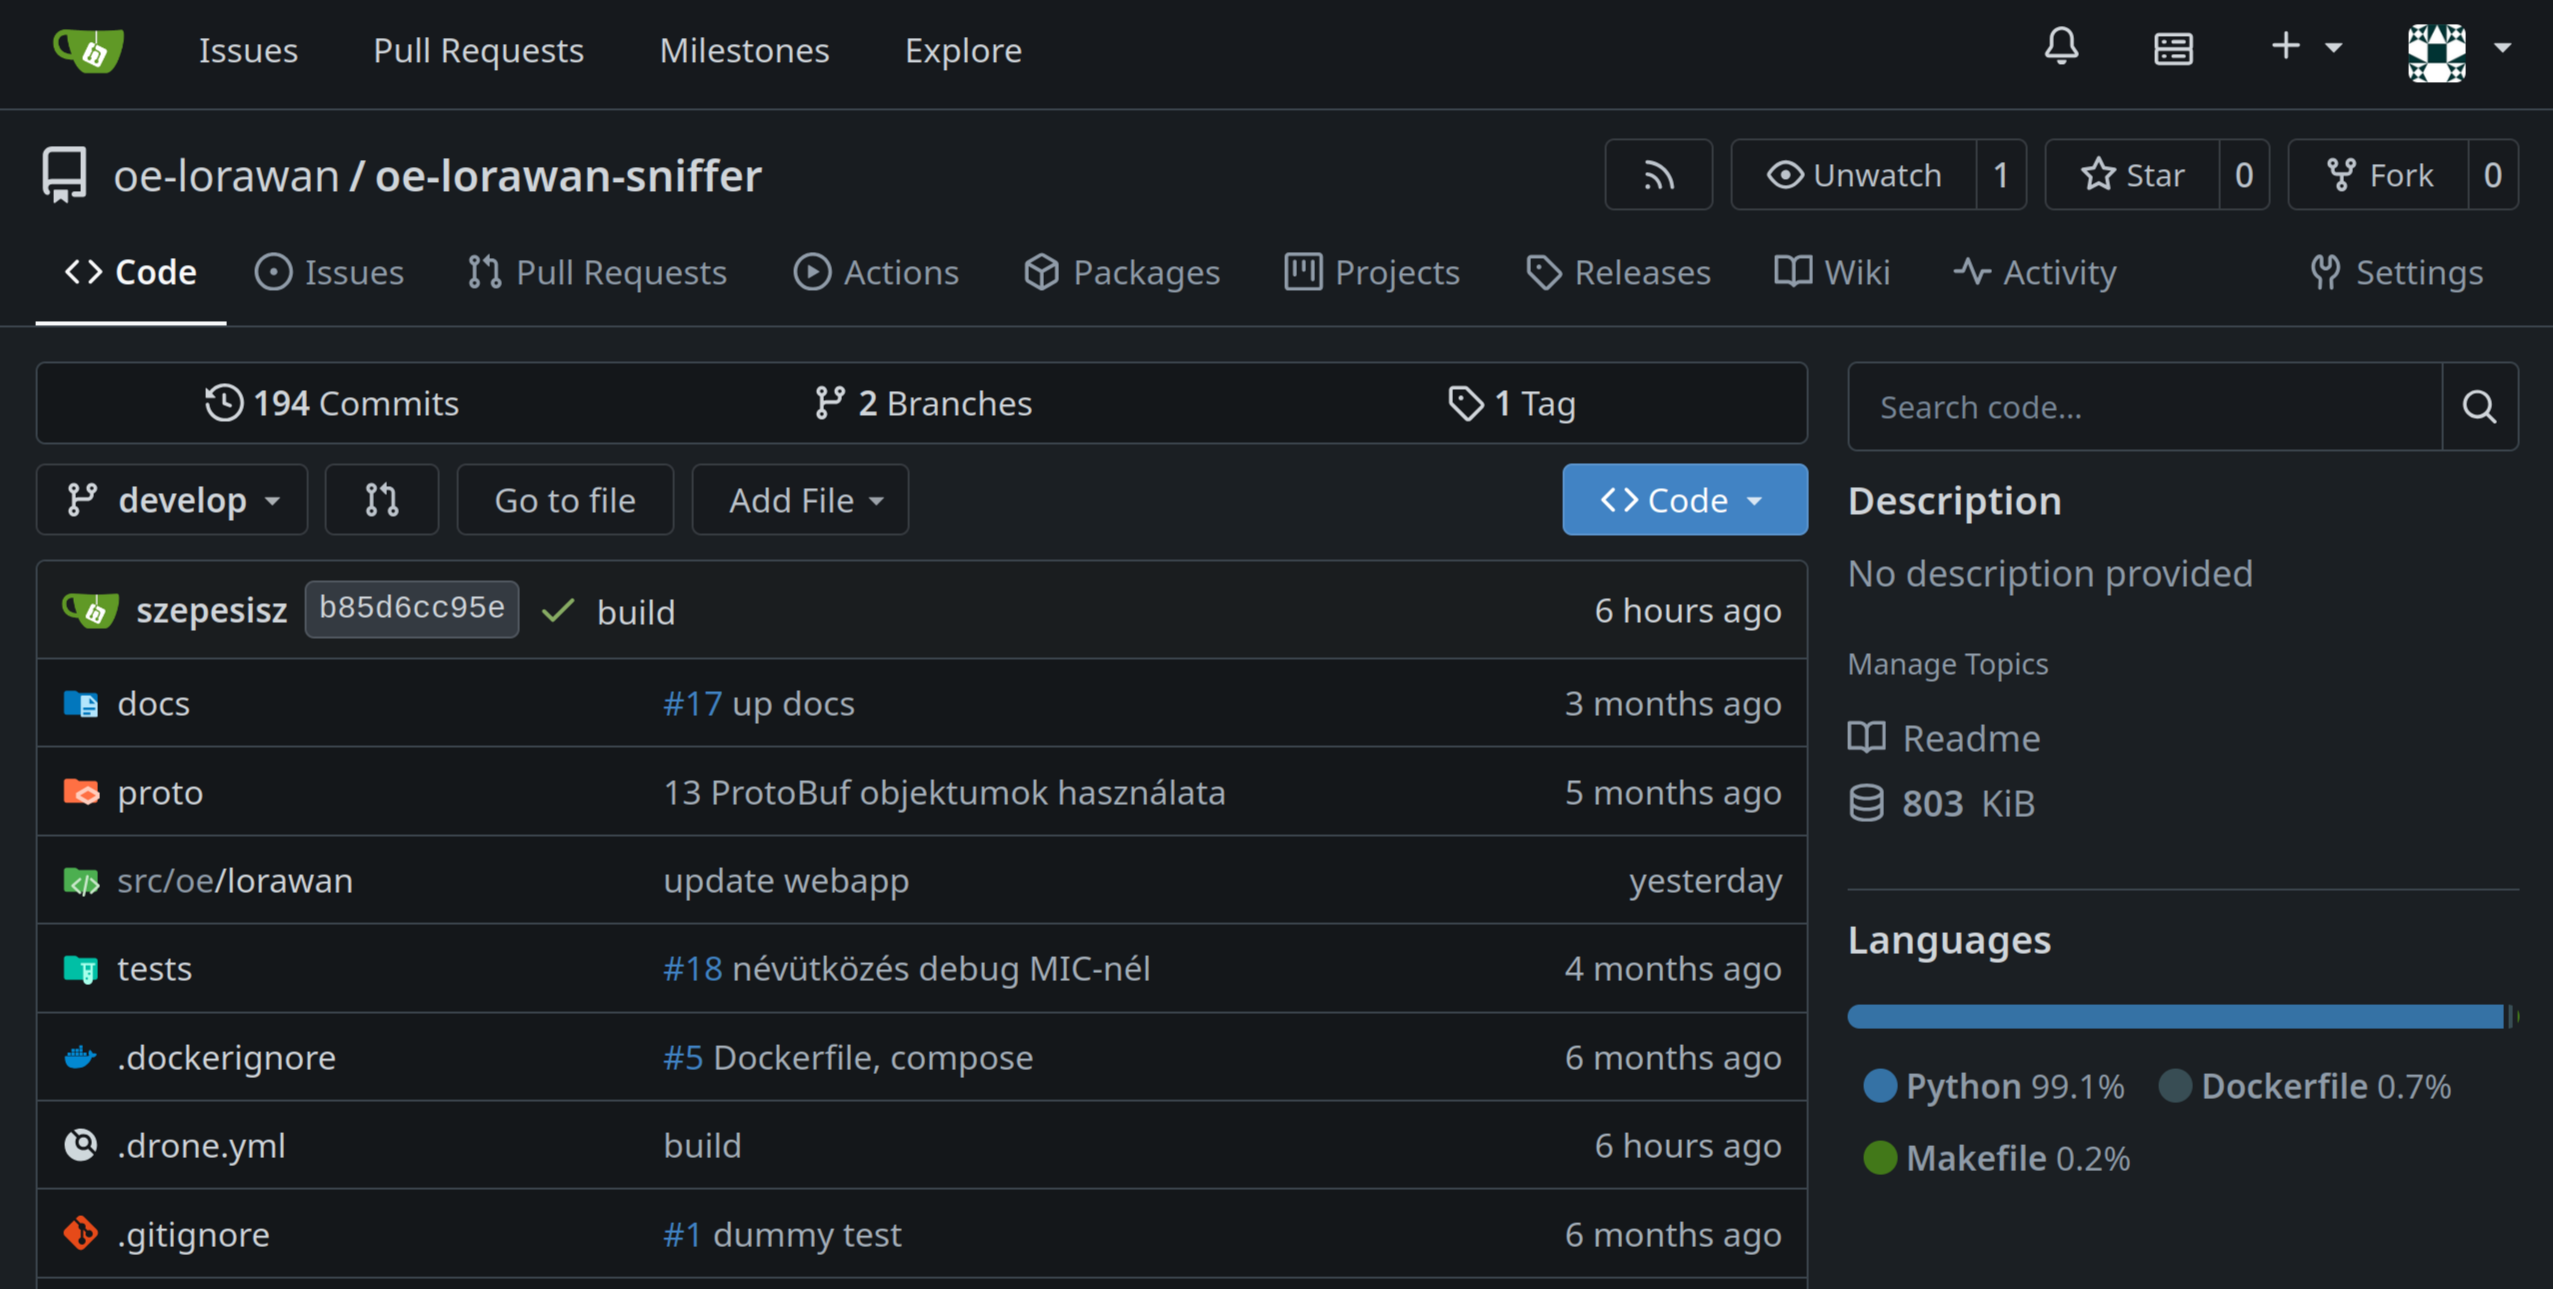
\includegraphics[width=1\linewidth]{img/gitea_sniffer.png}
	\caption{A manage-elt service repo-ja a Gitea-n}
	\label{fig:seq}
\end{figure}

\subsection{A kezelt service}

A kód maga egy digital twin modell alapú eszköz, amely a hálózati forgalmat figyelve leköveti a fizikai hardware-ek állapotait, ezzel lehetővé téve azoknak kiberbiztonsági analízisét.

A kód moduláris felépítésű, így nemcsak valós idejű forgalom figyelésére alkalmas, hanem alkalmi interakció is lehetséges vele REST API-n keresztül, melynek Swagger felülete felhasználói használatot is lehetővé tesz.

A Dockerfile, amely segítségével Python kódból Docker image-et készül, multistage build-et használ. Kiaknázva, hogy a kód Python package-ként van fejlesztve (pip-pel telepíthető, abból wheel készíthető), első lépésként egy wheel-t készít. A verziószámot a setuptools-scm segítségével a git tagből számolja dinamikusan, így minden állapot új verziószámot kap. Ehhez van szükség a git-re.

\begin{lstlisting}
FROM python:${PYTHON_VERSION}-slim AS base
ENV PIP_ROOT_USER_ACTION=ignore
RUN apt-get update && \
    yes | apt-get install git && \
    pip install build
COPY . .
RUN python -m build .

FROM python:${PYTHON_VERSION}-slim AS wheel
ENV PIP_ROOT_USER_ACTION=ignore
COPY --from=base dist/*.whl .
\end{lstlisting}

A build lépésbe már csak a wheel-t hozzom át, a git-re, a build csomagra és a az apt indexére nincs szükség:

\begin{lstlisting}
FROM wheel AS build
RUN pip install $(find ./*.whl)  && \
    rm $(find ./*.whl) && \
    mkdir /app
WORKDIR /app
ENV PYTHONBUFFERED=1
ENTRYPOINT ["app"]
\end{lstlisting}

A pyproject.toml metaadat-leíróban project scriptként az "app" is meg van adva, így ez a Dockerfile akár módosítás nélkül felhasználható majd a kutatócsoport többi komponensénél is.

A tesztelést a build lépéstől folytatja, így nemcsak a véglegeshez hasonló, hanem pontosan azt a kódod teszteli, amely majd a containerben futni fog, így csökkentve a hibák elfedődésének kockázatát:

\begin{lstlisting}
FROM build AS test
WORKDIR /
COPY --from=base . .
RUN python \
        -m pip install \
            -r requirements_test.txt  \
            pytest pytest-cov \
            bandit ruff \
    && mkdir \
        -p testresults \
    && python \
        -m pytest \
            --junitxml testresults/unittests.junit.xml \
            --cov-report xml:testresults/coverage.xml \
            --color=no \
        || true \
    && python \
        -m bandit \
            --exit-zero \
            -r \
            -f xml \
            src \
        > testresults/bandit.junit.xml \
    && python \
        -m ruff check \
            --exit-zero \
            src \
        > testresults/ruff.junit.xml
\end{lstlisting}


\subsection{Drone CI}

A Drone platform szorosan integrálódik a Gitea-val, így míg oda külön felhasználókat kell felvenni, a Drone a Gitea-n keresztül authentikál, OAuth2 alkalmazásként:


\begin{figure}[H]
	\centering
	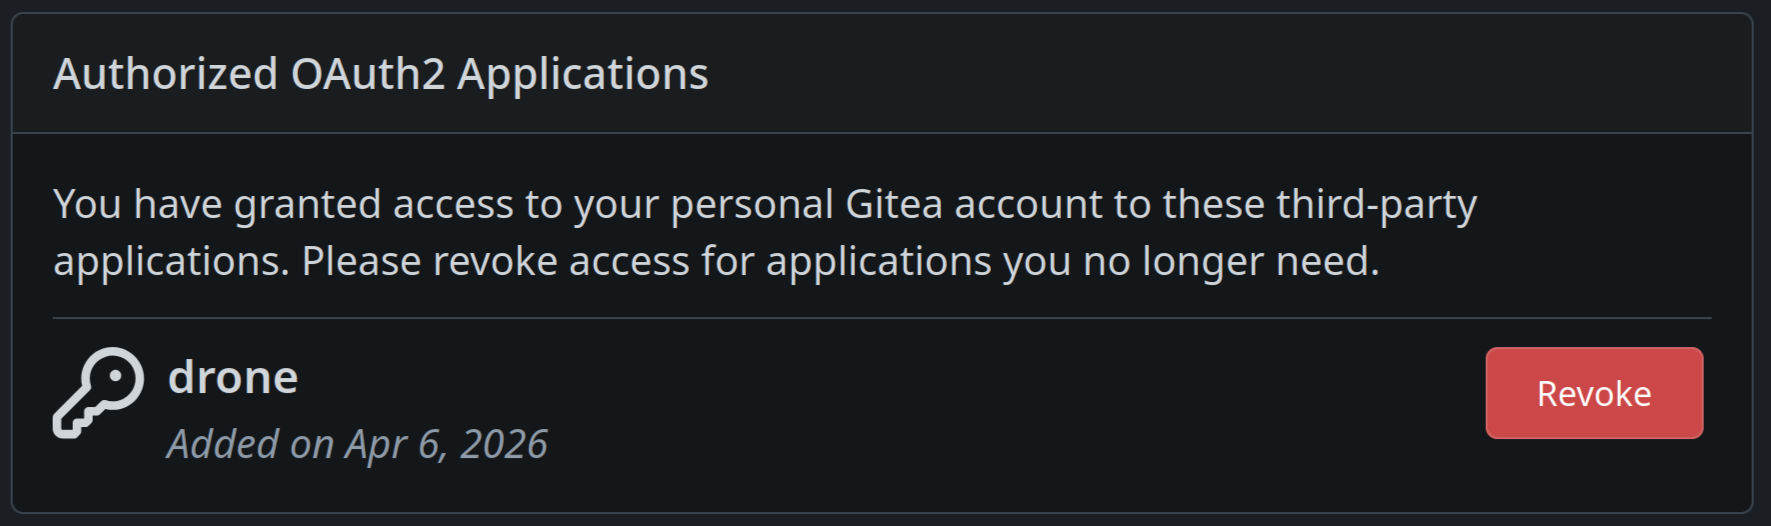
\includegraphics[width=0.7\linewidth]{img/gitea_oauth.png}
	\caption{A Drone alkalmazás a Gitea-n}
	\label{fig:seq}
\end{figure}

A létrehozáskor kapott, és megadott azonosítókat a Drone service-nél környezeti változóként adjuk meg, ahova szintén külső, .env fileból kerülnek:

\begin{lstlisting}
drone:
    image: drone/drone:${DRONE_VERSION:-latest}
    container_name: drone
    environment:
      DRONE_GITEA_SERVER: http://gitea:3000
      DRONE_GITEA_CLIENT_ID: ${DRONE_GITEA_CLIENT_ID}
      DRONE_GITEA_CLIENT_SECRET: ${DRONE_GITEA_CLIENT_SECRET}
      DRONE_RPC_SECRET: ${DRONE_RPC_SECRET}
      DRONE_USER_CREATE: username:szepesisz,admin:true
      DRONE_SERVER_HOST: localhost:8102
      DRONE_SERVER_PROTO: http
    ...
\end{lstlisting}

\subsubsection{Drone Runner Docker}

A tényleges pipeline futtatást egy drone-runner-docker példány végzi, akinek a Drone-nal való kommunikációhoz meg kell adni a secretet, amit fent is megadtunk:

\begin{lstlisting}
  drone-runner:
    image: drone/drone-runner-docker:${DRONE_DOCKER_RUNNER_VERSION:-latest}
    container_name: drone-runner
    environment:
      DRONE_RPC_PROTO: http
      DRONE_RPC_HOST: drone:80
      DRONE_RPC_SECRET: ${DRONE_RPC_SECRET}
    volumes:
      - /var/run/docker.sock:/var/run/docker.sock
\end{lstlisting}

Itt is mount-oljuk a Docker socketet. Erre a pipeline lépések image-einek eléréséhez mindenképp szükség van ennél a típusú runnernél. De mivel Docker buildet szeretnénk automatizálni, egy docker-in-docker (dind) megoldás is szükséges. Ehhez egy admin userre volt szükség a Drone felületen (DRONE\_USER\_CREATE), hogy a forráskód repóját Trusted-nak jelölhessem, ugyanis csak ekkor megoldható a dind build.

\subsubsection{A pipeline}

A folyamatot egy .drone.yml fileban definiáljuk.

\begin{lstlisting}
kind: pipeline
type: docker
name: default

...

volumes:
  - name: docker
    host:
      path: /var/run/docker.sock
\end{lstlisting}

A kezdeti clone-ozást a lokális elérés miatt felül kell definiálni, valamint a tag-ekre is szükség lesz a verzió meghatározásához:

\begin{lstlisting}

clone:
  disable: true

steps:
- name: clone
  image: alpine/git
  commands:
  - git clone http://192.168.0.173:8101/oe-lorawan/oe-lorawan-sniffer.git .
  - git fetch --tags
  - git checkout $DRONE_COMMIT

...
\end{lstlisting}


A tesztlépéseket nem a pipeline-ban, hanem a Dockerfile-ban definiáljuk, így hordozhatóbb a megoldás, akár lokálisan is könnyen használható.

\begin{lstlisting}
- name: test
  image: docker:24.0
  privileged: true
  commands:
  - docker build --target test .

  volumes:
    - name: docker
      path: /var/run/docker.sock
\end{lstlisting}

Majd maga a build következik:

\begin{lstlisting}
- name: build
  image: docker:24.0
  privileged: true
  commands:
  - docker build --tag oe-lorawan/oe-lorawan-sniffer --target build .
  - docker tag oe-lorawan/oe-lorawan-sniffer oe-lorawan/oe-lorawan-sniffer:$(docker run oe-lorawan/oe-lorawan-sniffer --version)
  - docker tag oe-lorawan/oe-lorawan-sniffer oe-lorawan/oe-lorawan-sniffer:latest

  volumes:
    - name: docker
      path: /var/run/docker.sock
\end{lstlisting}

Mivel a "build" target előzménye a "test"-nek, ez a lépés a cache-elés miatt hatékonyan fut le.

Itt kihasználjuk, hogy az alkalmazás a --version flaggel képes megmondani a saját verzióját.

Ugyanezek a lépések a fejlesztőnek Makefile-ként is elérhetők, ugyanazzal a Dockerfile-lal:

\begin{lstlisting}
DOCKER_USERNAME = oe-lorawan
APPLICATION_NAME = oe-lorawan-sniffer

IMAGE = ${DOCKER_USERNAME}/${APPLICATION_NAME}

DOCKER_EXEC = sudo docker

build:
	${DOCKER_EXEC} build --tag ${IMAGE} --target build .
	${DOCKER_EXEC} tag ${IMAGE} ${IMAGE}:$$(sudo docker run ${IMAGE} --version)
	${DOCKER_EXEC} tag ${IMAGE} ${IMAGE}:latest


test: build
	${DOCKER_EXEC} build --target test .
\end{lstlisting}

Ezennel kész az új image, már csak a stacket kell frissíteni.

Erre Portainer Community Edition felületén elérhető webhook nem egészen alkalmas. Az ugyanis csak akkor frissítené a környezetet, ha az azt leíró repo változott, ami nálunk nem áll fenn. Az erőltett frissítés Business Edition feature.

Azonban a grafikus felületen van rá gomb, tehát az API hívást kell kihasználni:

\begin{lstlisting}
- name: deploy
  image: curlimages/curl:8.17.0
  secrets: [ portainer_api_key ]
  environment:
    PORTAINER_API_KEY:
      from_secret: portainer_api_key

  commands:
  - "curl -i -X PUT
     http://192.168.0.173:8100/api/stacks/2/git/redeploy?endpointId=1 -H
     \"X-API-KEY: $PORTAINER_API_KEY\" --json '{ \"ForceUpdate\": false }'"
\end{lstlisting}

Az authentikációhoz tokent hoztunk létre a Portainerben, amit a Drone-ban secretként tárolunk. A stack id beégetése finomítandó, ha esetleg több környezetet akarnánk kezelni, de demonstrációs célra elég volt.

\begin{figure}[H]
	\centering
	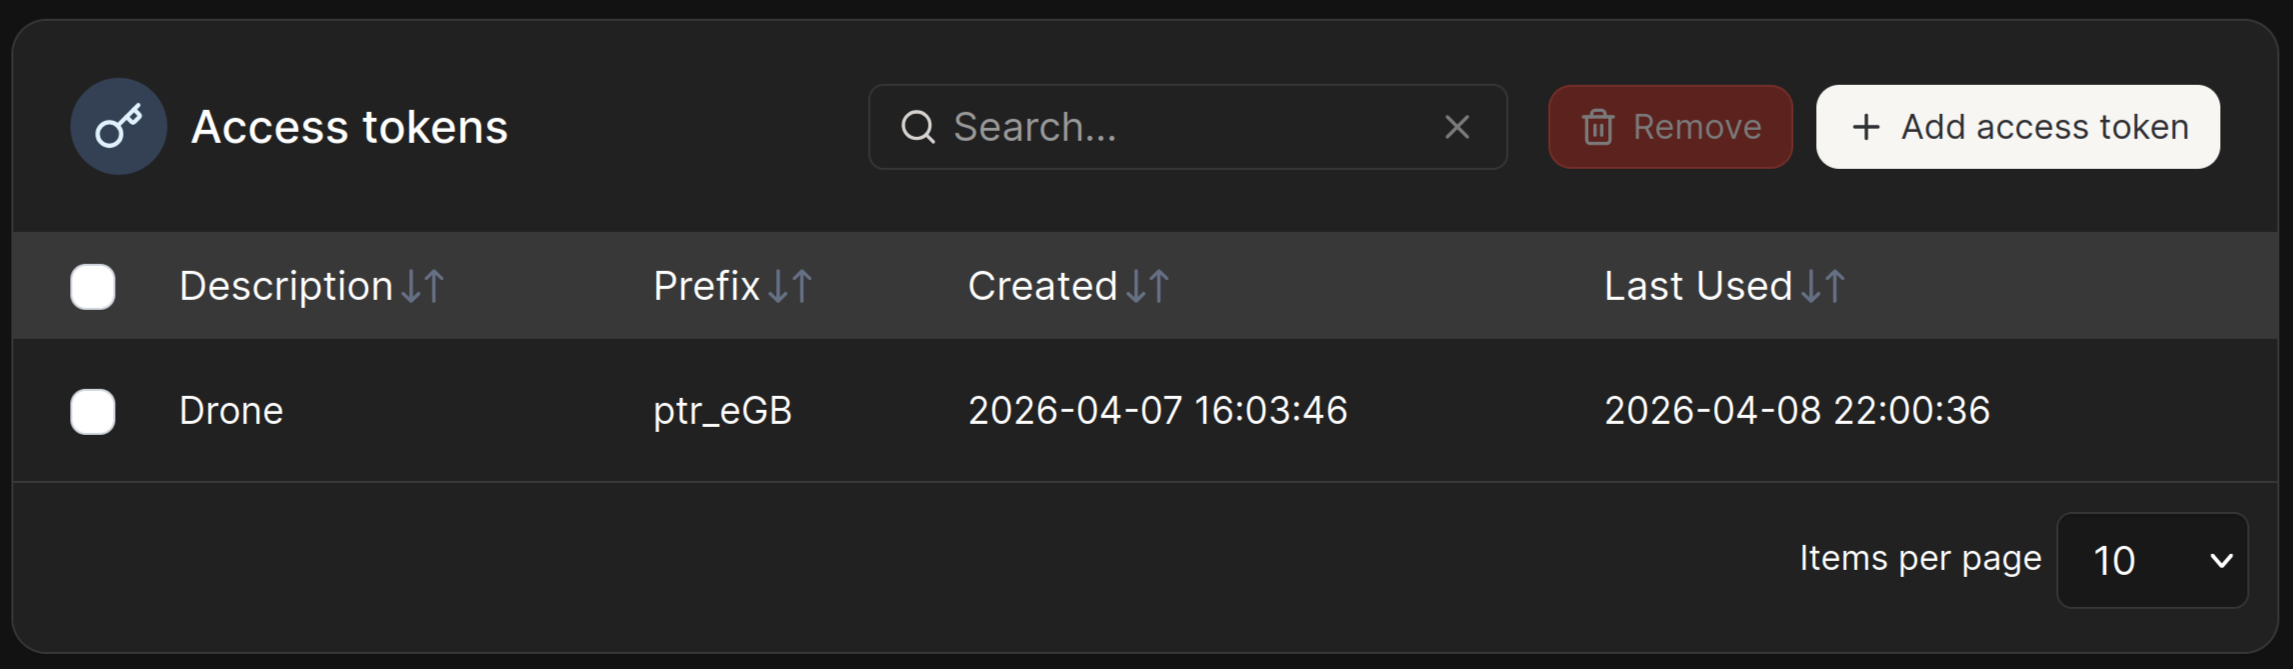
\includegraphics[width=0.7\linewidth]{img/portainer_token.png}
	\caption{Token a Portaineren a deploymenthez}
	\label{fig:seq}
\end{figure}


\begin{figure}[H]
	\centering
	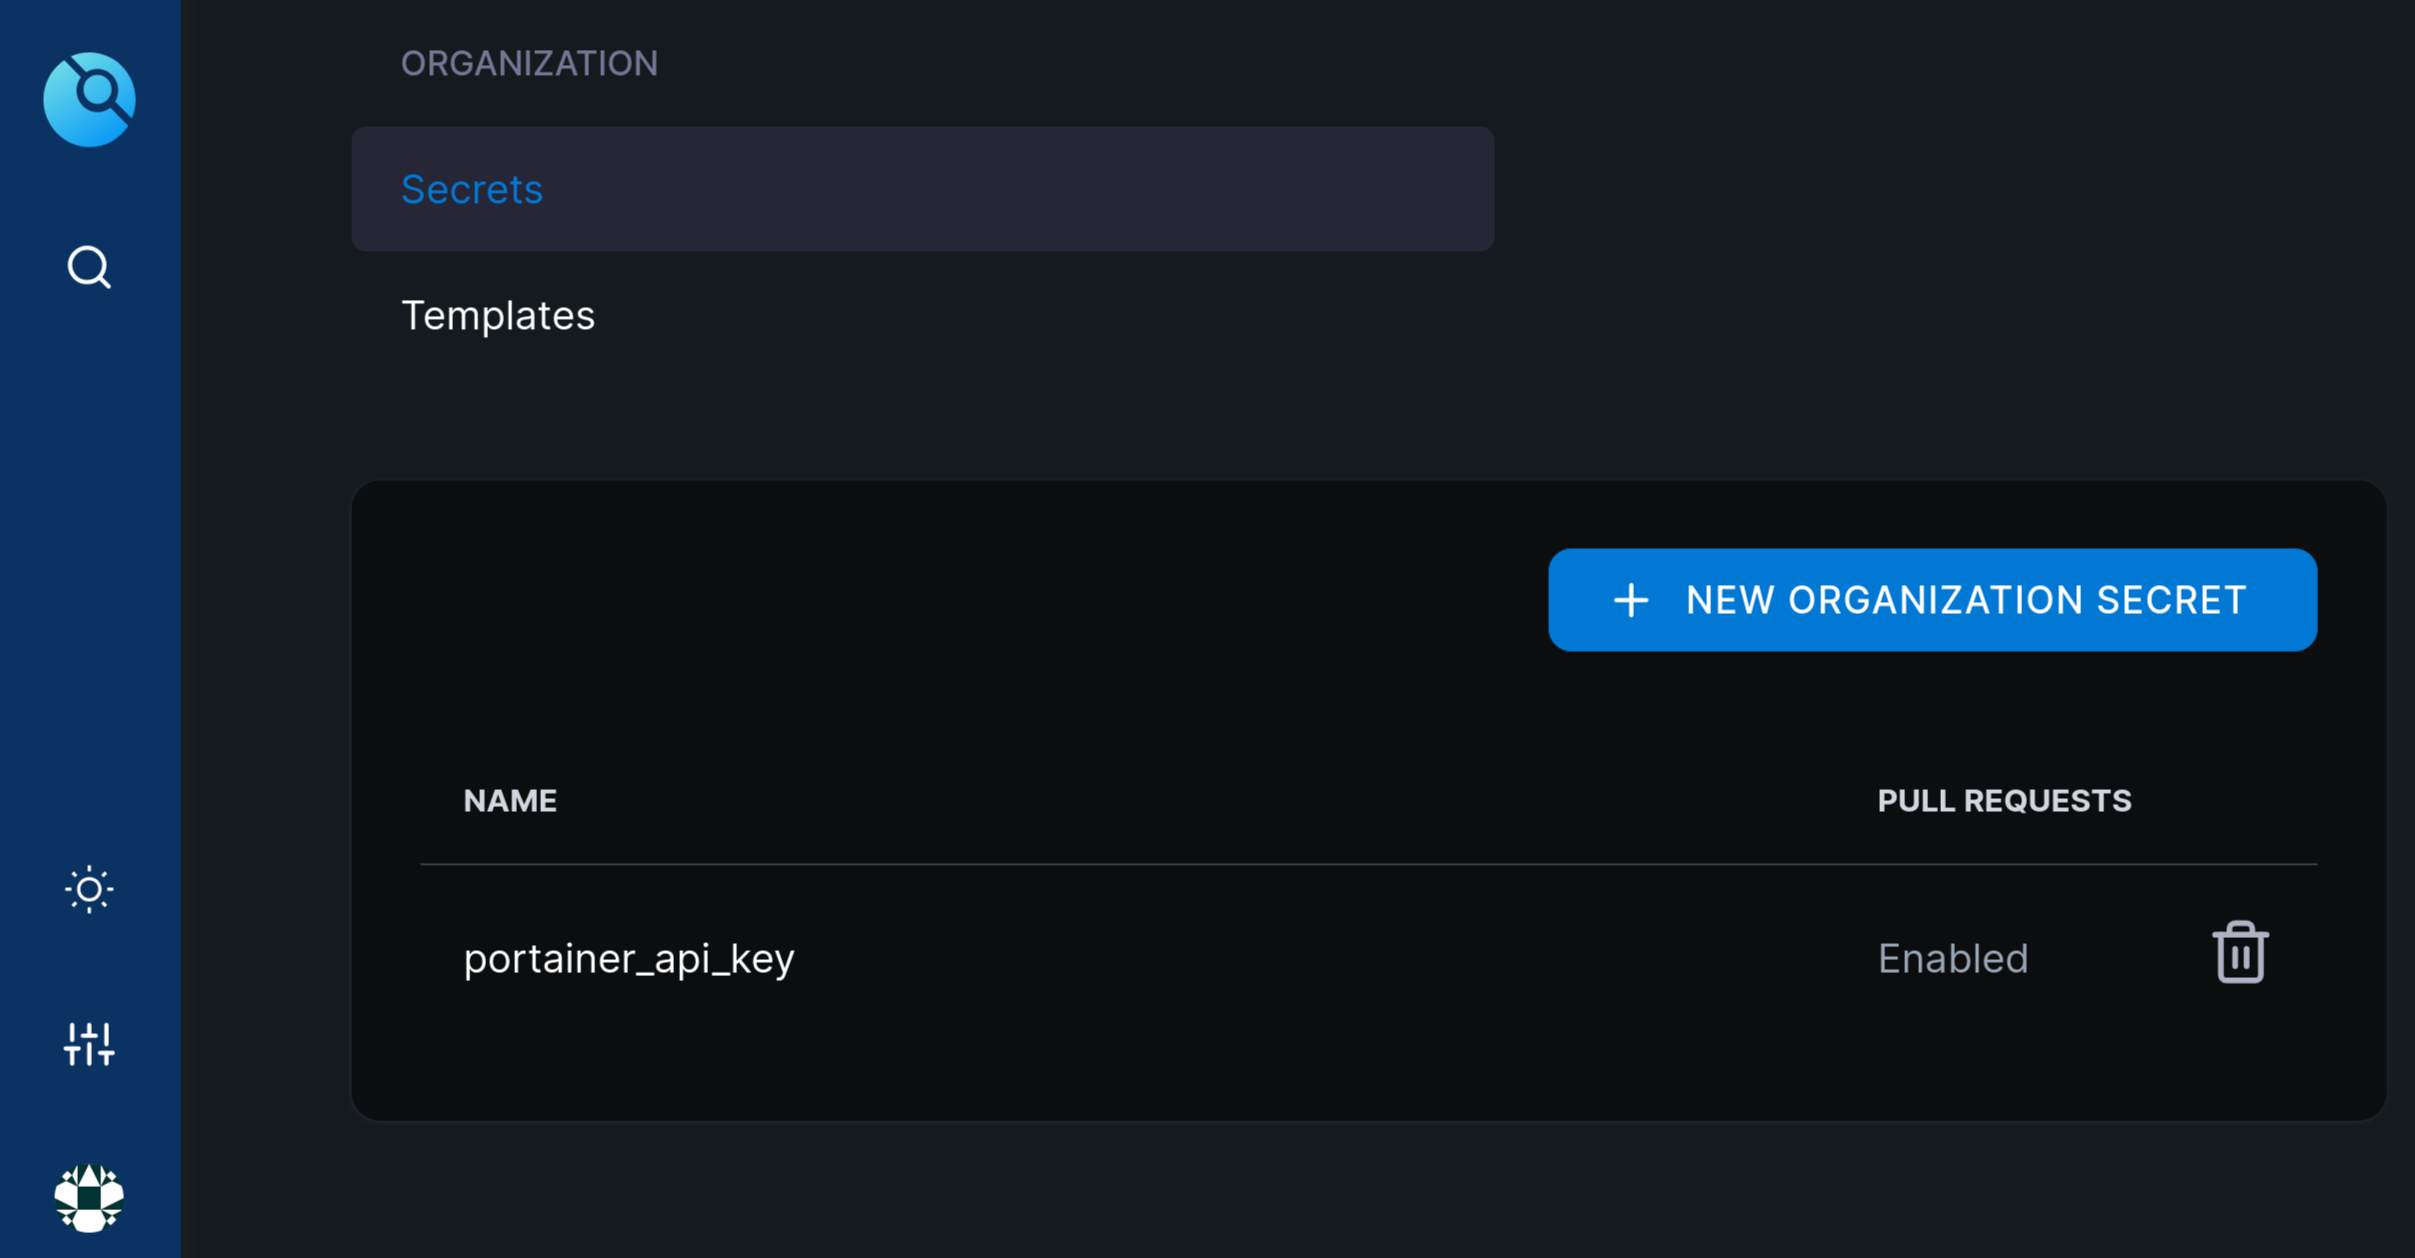
\includegraphics[width=0.7\linewidth]{img/portainer_token_drone.png}
	\caption{A Portaineren token a Drone felületen}
	\label{fig:seq}
\end{figure}

A sikeresen lefutott pipeline:

\begin{figure}[H]
	\centering
	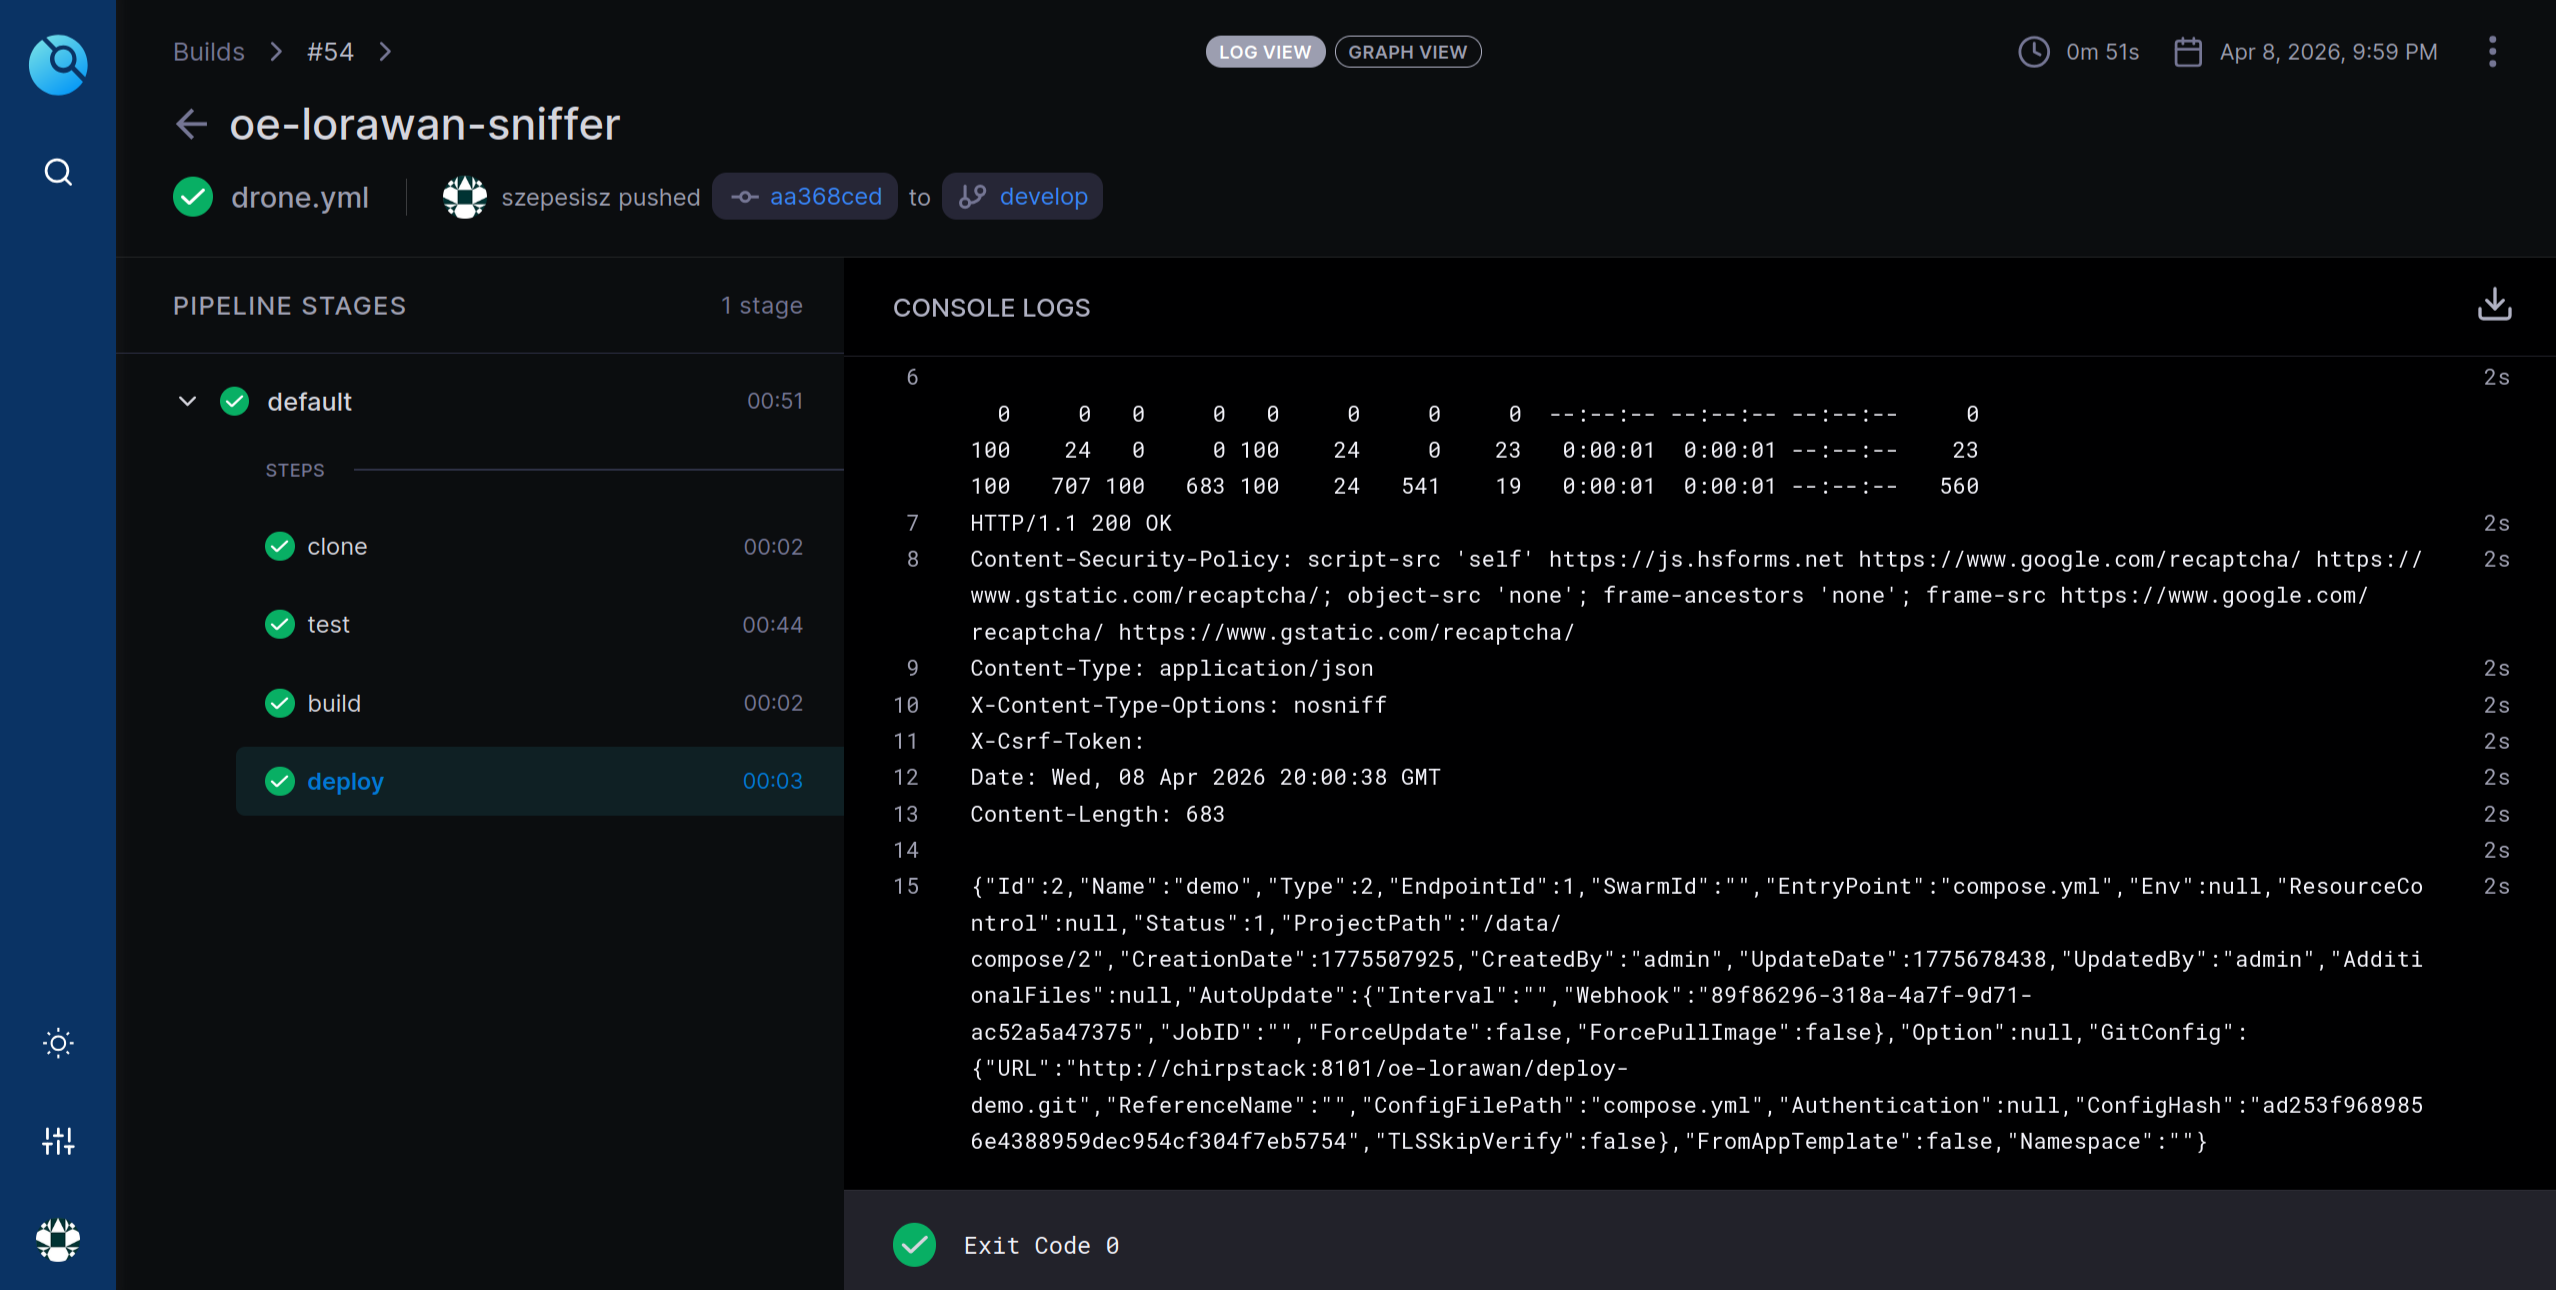
\includegraphics[width=1\linewidth]{img/drone_pipeline.png}
	\caption{A sikeresen lefutott pipeline}
	\label{fig:seq}
\end{figure}

Valamint a visszajelzés a Gitea felületen:

\begin{figure}[H]
	\centering
	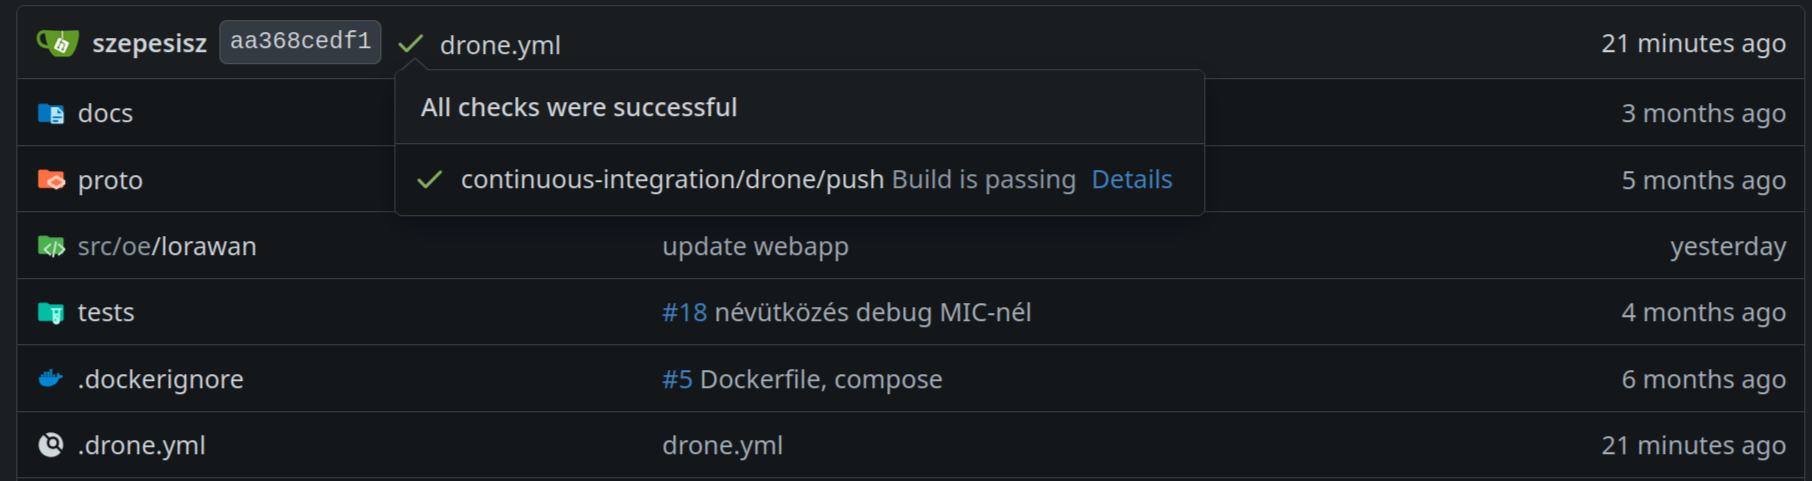
\includegraphics[width=1\linewidth]{img/gitea_feedback.png}
	\caption{Gitea visszajelzés}
	\label{fig:seq}
\end{figure}


